\documentclass[25pt, a2papper, portrait]{tikzposter}
\usepackage[brazil]{babel}
\usepackage[utf8]{inputenc}
\usepackage{color}
\usepackage{mathtools}
\usepackage{diagbox}
\usepackage{colortbl}

\definecolor{NavyBlue}{rgb}{0, 0, 0.5}

\newcolumntype{P}[1]{>{\centering\arraybackslash}p{#1}}

\title{\parbox{\linewidth}{\centering\textcolor{NavyBlue}{Reconhecimento de Entidades Mencionadas em Notificações de
  Atos de Concentração do Conselho Administrativo de Defesa Econômica}}}
\author{%
\begin{minipage}{\linewidth}
  \centering
  \begin{minipage}{.75\linewidth}
  \hspace*{15.5cm} Renan Fichberg \\
  \hspace*{7.5cm} Orientador: Prof. Dr. Marcelo Finger
  \end{minipage}\hfill
\end{minipage}%
}
\institute{%
\begin{minipage}{\linewidth}
  \centering
  \begin{minipage}{1\linewidth}
  \hspace*{8.75cm} Universidade de São Paulo, Instituto de Matemática e Estatística \\
  \hspace*{10.25cm} \large{\texttt{renan.fichberg@usp.br --- https://linux.ime.usp.br/\~{}fichberg/mac0499/}}
  \end{minipage}\hfill
\end{minipage}%
}

\makeatletter
\newcommand\insertlogoi[2][]{\def\@insertlogoi{\includegraphics[#1]{#2}}}
\newcommand\insertlogoii[2][]{\def\@insertlogoii{\includegraphics[#1]{#2}}}
\newlength\LogoSep
\setlength\LogoSep{55pt}

\insertlogoi[width=11.2cm]{usp.png}
\insertlogoii[width=11.2cm]{imeusp.png}

\renewcommand\maketitle[1][]{  % #1 keys
    \normalsize
    \setkeys{title}{#1}
    % Title dummy to get title height
    \node[transparent,inner sep=\TP@titleinnersep, line width=\TP@titlelinewidth, anchor=north, minimum width=\TP@visibletextwidth-2\TP@titleinnersep]
        (TP@title) at ($(0, 0.5\textheight-\TP@titletotopverticalspace)$) {\parbox{\TP@titlewidth-2\TP@titleinnersep}{\TP@maketitle}};
    \draw let \p1 = ($(TP@title.north)-(TP@title.south)$) in node {
        \setlength{\TP@titleheight}{\y1}
        \setlength{\titleheight}{\y1}
        \global\TP@titleheight=\TP@titleheight
        \global\titleheight=\titleheight
    };

    % Compute title position
    \setlength{\titleposleft}{-0.5\titlewidth}
    \setlength{\titleposright}{\titleposleft+\titlewidth}
    \setlength{\titlepostop}{0.5\textheight-\TP@titletotopverticalspace}
    \setlength{\titleposbottom}{\titlepostop-\titleheight}

    % Title style (background)
    \TP@titlestyle

    % Title node
    \node[inner sep=\TP@titleinnersep, line width=\TP@titlelinewidth, anchor=north, minimum width=\TP@visibletextwidth-2\TP@titleinnersep]
        at (0,0.5\textheight-\TP@titletotopverticalspace)
        (title)
        {\parbox{\TP@titlewidth-2\TP@titleinnersep}{\TP@maketitle}};

    \node[inner sep=0pt,anchor=west]
      at ([xshift=-\LogoSep]title.west)
      {\@insertlogoi};

    \node[inner sep=0pt,anchor=east]
      at ([xshift=\LogoSep]title.east)
      {\@insertlogoii};

    % Settings for blocks
    \normalsize
    \setlength{\TP@blocktop}{\titleposbottom-\TP@titletoblockverticalspace}
}
\makeatother

\begin{document}

\maketitle

\block{Introdução}
{
O Conselho Administrativo de Defesa Econômica (CADE) é um orgão independente que reporta ao Ministério da Justiça e possui como missão garantir a livre
concorrência de mercado em todo o território Brasileiro e realiza as suas funções legais de acordo com a Lei Nº 12.529/2011.
O CADE dispõem de uma base de dados bastante extensa, com processos judiciais de vários tipos distintos datados do ano de 1980 até os dias atuais e mais de 100 tipos diferentes de
documentos, desde formulários, notificações de processos e cópias escaneadas de documentos diversos até arquivos de áudio e vídeo.

Os processos judiciais objetos de estudo deste trabalho são os denominados Atos de Concentração. Um dado Ato de Concentração submetido ao Conselho Administrativo de Defesa
Econômica pode ser analisado sob dois diferentes ritos: sumário ou ordinário. Em particular, o objetivo do trabalho desenvolvido foi de extrair o máximo de informações potencialmente
relevantes para uma futura tentativa de classificação automatizada do tipo de rito que um dado futuro Ato de Concentração poderá seguir. Para isso, foi desenvolvido um
córpus composto de cinqüenta Atos de Concentração do ano de 2016 com anotações de entidades mencionadas predefinidas usando conhecimento e técnicas de processamento de linguagem natural
e ferramentas de aprendizado de máquina supervisionado.
}

\begin{columns}
    \column{0.3}
    \block{Atos de Concentração}{
    Os Atos de Concentração Econômicas (AC) são caracterizados por operações que envolvem duas ou mais empresas independentes, conforme descrito no artigo 90 da Lei 12.529/2011.
    Tais operações podem ser aquisições de controle ou incorporações de uma ou mais empresas por outras ou ainda a celebração de contratos associativos, consórcios
    ou \textit{joint ventures} entre empresas. A natureza destas operações, aliadas ao faturamento bruto anual ou volume de negócios no Brasil dos agentes
    econômicos envolvidos, que justificam a existência dos ACs analisados pelo CADE. Quando o faturamento bruto anual de uma das empresas envolvidas na
    operação atinge o patamar mínimo de R\$ 750 milhões e o de uma outra, também envolvida na operação, o patamar de R\$ 75 milhões, o AC deve ser notificado ao CADE.
    Os possíveis tipos de operações que um AC pode ter são:
    \begin{itemize}
      \item \textbf{Fusão}: união de duas ou mais empresas distintas para formar um novo agente econômico único.
      \item \textbf{Incorporação}: ato de uma ou mais empresas incorporar total ou parcialmente outras empresas dentro de uma mesma pessoa jurídica,
      de tal forma que o incorporado desaparece como pessoa jurídica, mas o incorporador mantém a sua identidade jurídica após a operação.
      \item \textbf{Aquisição}: ato de uma empresa adquirir o controle total ou parcial da participação acionária de outra empresa.
      \item \textbf{\textit{Joint venture}}: criação de uma nova empresa a partir da associação entre duas ou mais empresas, de tal forma
      que as empresas que se associaram mantém normalmente suas identidades jurídicas pós operação.
    \end{itemize}

    }
    \block{Métricas}{
    Foram utilizadas para medir o desempenho do córpus as seguintes métricas:

    \vspace*{0.25cm}
    A precisão (\textbf{P}):
    \vspace*{0.25cm}
    \begin{equation}
     \nonumber
     \text{\textbf{P}} = \dfrac{\text{\#itens relevantes recuperados}}{\text{\#itens recuperados}} = \dfrac{\text{\textbf{VP}}}{\text{\textbf{VP} + \textbf{FP}}}
    \end{equation}
    A cobertura (\textbf{C}):
    \vspace*{0.25cm}
    \begin{equation}
     \nonumber
     \text{\textbf{C}} = \dfrac{\text{\#itens relevantes recuperados}}{\text{\#itens relevantes}} = \dfrac{\text{\textbf{VP}}}{\text{\textbf{VP} + \textbf{FN}}}
    \end{equation}
    A medida-F balanceada (\textbf{F}$_1$):
    \vspace*{0.25cm}
    \begin{equation}
    \nonumber
     \text{\textbf{F}}_1 = \dfrac{2\text{\textbf{PC}}}{\text{\textbf{P}} + \text{\textbf{C}}}
    \end{equation}

    \vspace*{0.5cm}

    Onde \textbf{VP}, \textbf{FP}, \textbf{FN} e \textbf{VN} significam Verdeiro Positivo, Falso Positivo, Falso Negativo e Verdeiro Negativo, respectivamente.
    }

    \column{0.7}
    \block{Córpus}{
    Problemas de processamento de linguagem natural envolvem o entendimento de linguagens naturais por parte das máquinas ou mesmo geração de linguagem natural (isto é, a conversão
    de uma representação entendida por computadores em uma representação em linguagem natural). Este trabalho se encaixa na primeira categoria de tal
    modo que foi desenvolvido um córpus (um conjunto de textos selecionados), posteriormente anotado manualmente, para gerar um modelo de treinamento capaz de extrair informações
    de forma automatizada. Foram considerados os seguintes pontos na criação do córpus:
    \begin{itemize}
      \item \textbf{Linguagem}: No caso, português.
      \item \textbf{Estrutura}: Forma que as notificações dos Atos de Concentração são estruturadas.
      \item \textbf{Representatividade}: Os Atos selecionados precisam constituir de uma amostra representativa da população de interesse.
      \item \textbf{Tamanho}: Precisa ser suficientemente extenso. O córpus construído tem pouco mais de 50000 palavras.
    \end{itemize}
    }

    \block{Reconhecimento de Entidades Mencionadas}{
    Uma entidade mencionada (EM) é um objeto do mundo real que possui um nome próprio, como por exemplo uma pessoa ou uma organização. As entidades mencionadas do
    córpus foram anotadas por meio de uma ferramenta \textit{web} chamada BRAT, v.1.3.0, um projeto \textit{open source} (Licença MIT) recente, desenvolvido colaborativamente por
    pesquisadores de vários grupos distintos com interesse em anotações de texto. Na Figura 1 abaixo, anotações BRAT em uma sentença de um Ato de Concentração:
    \begin{tikzfigure}
        \hspace*{-0.5cm}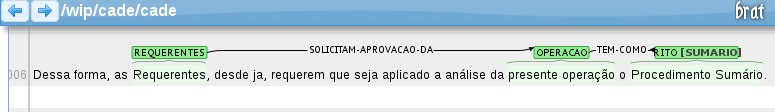
\includegraphics[width=0.6\textwidth]{bratposter.png}
    \end{tikzfigure}
    \begin{center}
      Figura 1: Anotações manuais de entidades mencionadas no BRAT de um dado Ato de Concentração.
    \end{center}
    Foram usados também os módulos de treinamento e reconhecimento de entidades mencionadas do Apache OpenNLP v.1.6.0. Porém, devido à necessidade de modelos de
    tokenização e de detecção de sentenças para poder treinar um modelo de reconhecimento de entidades mencionadas, foram usados modelos previamente gerados sobre o córpus
    Amazônia (possivelmente o córpus em português mais revisado por especialistas e bastante extenso).

    O processo de tokenização consiste em quebrar o texto em \textit{tokens} (palavras, números e pontuações, basicamente) enquanto o de detecção de sentenças consiste em quebrar
    o texto em sentenças, como os nomes sugerem. Assim, a sentença apresentada na Figura 1 acima é tokenizada da seguinte maneira:

    \begin{minipage}{\linewidth}
      \centering
      \begin{minipage}{.75\linewidth}
      \Large{``}\fbox{Dessa} \fbox{forma} \fbox{,} \fbox{as} \fbox{Requerentes} \fbox{,} \fbox{desde} \fbox{já} \fbox{,} \fbox{requerem} \fbox{que} \fbox{seja} \fbox{aplicado} \fbox{a}
      \fbox{análise} \fbox{da} \fbox{presente} \fbox{operação} \fbox{o} \fbox{Procedimento} \fbox{Sumário} \fbox{.}"
      \end{minipage}\hfill
    \end{minipage}%

    \vspace*{-0.2cm}
    }

    \block{Resultados}
    {
    Resultados da validação cruzada com o método \textit{holdout}. Cada $C_i$ representa uma combinação de grupos de teste e de treinamento compostos
    por cinco e quarenta e cinco Atos de Concentração, respectivamente. Os rótulos \textit{L} são apresentados na primeira coluna.

      \begin{center}
      \begin{tabular}{| P{4cm} | P{3cm} | P{3cm} | P{3cm} | P{3cm} | P{3cm} | P{3cm} | P{3cm} | P{3cm} | P{3cm} | P{3cm} |}
        \hline
        \backslashbox[45mm]{\textit{L}}{$C_i$} & $C_1$ & $C_2$ & $C_3$ & $C_4$ & $C_5$ & $C_6$ & $C_7$ & $C_8$ & $C_9$ & $C_{10}$ \\
        \hline
        \small{\textbf{R}}                 & \small{327} & \small{263} & \small{218} & \small{324} & \small{293} & \small{210} & \small{270} & \small{263} & \small{220} & \small{243} \\ \hline
        \small{\textbf{T}}                 & \small{774} & \small{527} & \small{491} & \small{741} & \small{653} & \small{520} & \small{702} & \small{623} & \small{587} & \small{605} \\ \hline
        \small{\textbf{A}}   & \small{258} & \small{208} & \small{168} & \small{248} & \small{231} & \small{162} & \small{208} & \small{210} & \small{179} & \small{184} \\ \hline
        \small{\textbf{E1} + \textbf{E3}} & \small{461 + 55} & \small{272 + 47} & \small{286 + 37} & \small{431 + 62} & \small{379 + 43} & \small{323 + 35} & \small{443 + 51} & \small{371 + 42} & \small{375 + 33} & \small{375 + 46} \\ \hline
        \small{\textbf{E2} + \textbf{E3}} & \small{14 + 55} & \small{8 + 47} & \small{13 + 37} & \small{14 + 62} & \small{19 + 43} & \small{13 + 35} & \small{11 + 51} & \small{11 + 42} & \small{8 + 33} & \small{13 + 46} \\ \hline\hline
        \small{\textbf{P}} & \small{0.789} & \small{0.790} & \small{0.770} & \small{0.765} & \small{0.788} & \small{0.771} & \small{0.770} & \small{0.798} & \small{0.813} & \small{0.757} \\ \hline
        \small{\textbf{C}} & \small{0.333} & \small{0.394} & \small{0.342} & \small{0.334} & \small{0.353} & \small{0.311} & \small{0.296} & \small{0.337} & \small{0.305} & \small{0.304} \\ \hline
        \small{\textbf{F$_1$}} & \small{0.468} & \small{0.525} & \small{0.473} & \small{0.465} & \small{0.487} & \small{0.443} & \small{0.427} & \small{0.473} & \small{0.443} & \small{0.433} \\ \hline
      \end{tabular}
      \end{center}

      \begin{center}
      \begin{tabular}{| l | l |}
        \arrayrulecolor{white}\hline
        R: & EMs recuperadas \\ \hline
        T: & EMs existentes na coleção \\ \hline
        A: & EMs corretamente recuperadas (VP) \\ \hline
      \end{tabular}
      \begin{tabular}{| l | l |}
        \arrayrulecolor{white}\hline
        E1: & EMs perdidas (FN) \\ \hline
        E2: & EMs classificadas erradas (FP) \\ \hline
        E3: & EMs imprecisas (FN e FP) \\ \hline
      \end{tabular}
      \begin{tabular}{| l | l |}
        \arrayrulecolor{white}\hline
        P: & Valor precisão \\ \hline
        C: & Valor cobertura \\ \hline
        F$_1$: & Valor medida-F balanceada \\ \hline
      \end{tabular}
      \end{center}

      \vspace*{-0.6cm}
    }

\end{columns}


\end{document}

% https://pt.sharelatex.com/learn/Posters
